\documentclass[11pt]{article}
\usepackage[margin=1in]{geometry}
\usepackage[T1]{fontenc}
\usepackage{mathptmx}
\usepackage{amsmath,amssymb,amsthm,mathtools}
\usepackage{graphicx}
\usepackage{booktabs}
\usepackage{multirow}
\usepackage[numbers,sort&compress]{natbib}
\usepackage{xcolor}
\usepackage{microtype}
\usepackage{tikz}
\usetikzlibrary{positioning,arrows.meta,fit,decorations.pathreplacing}
\usepackage{algorithm}
\usepackage{algpseudocode}
\usepackage[colorlinks=true,linkcolor=blue!50!black,citecolor=blue!50!black,urlcolor=blue!50!black]{hyperref}
\usepackage[capitalise,noabbrev]{cleveref}

\newtheorem{proposition}{Proposition}
\newtheorem{lemma}{Lemma}
\theoremstyle{definition}
\newtheorem{definition}{Definition}
\theoremstyle{remark}
\newtheorem{remark}{Remark}

\newcommand{\ket}[1]{\lvert #1\rangle}
\newcommand{\bra}[1]{\langle #1\rvert}
\newcommand{\tr}{\operatorname{Tr}}
\newcommand{\RGR}{R_{\mathrm{GR}}}
\newcommand{\nvec}{\hat{\boldsymbol{n}}}
\newcommand{\bsig}{\boldsymbol{\sigma}}

\title{\textbf{Order, Timing, and Feedback:\\ A Quantum-Probability Decision State for Role-Aware Agents}}

\author{%
Lalit Aditya R D\\[4pt]
\small Vellore Institute of Technology, Chennai, India
}

\date{\small Draft preprint --- November 2026}

\begin{document}
\maketitle

\begin{abstract}
Language-model agents increasingly stand in for human decision makers in surveys, organisational workflows, and city-scale simulations, yet they store decisions as text and expose no explicit model of how the \emph{order} and \emph{timing} of evaluations shape a choice. We propose a quantum-probability decision state: a compact, external memory in which each role and planning level holds a density matrix, evidence acts as rotations generated by non-commuting criterion operators, commitment is a L\"uders projection, and stored decisions drift toward a default under an open-system channel. Three ideas from adjacent literatures fill gaps in this picture. From quantum cognition we take the parameter-free QQ equality as a falsifiable test of order effects; from the theory of dynamical decay control we take an overlap law in which the drift rate of a stored decision equals the overlap between the spectrum of its information environment and the spectrum of its review schedule; and from linear quantum feedback networks we take proportional output feedback to keep coupled roles coordinated. We report four results. (i) A reanalysis of six published order-effect data sets reproduces the QQ test and shows that the QQ-constrained model attains the best AIC in four of six; it also shows that any model with one-dimensional ``yes'' subspaces is rejected, because human data violate the reciprocity $P(B\,|\,A)=P(A\,|\,B)$ that such models impose. (ii) In simulation, order sensitivity tracks the commutator norm between criterion axes (Pearson $r=0.86$). (iii) The overlap law predicts a \emph{decision Zeno} regime, in which reviews freeze a decision, and a \emph{decision anti-Zeno} regime, in which reviews at an interval near the environment's correlation time more than double the drift rate ($2.11\times$); it also predicts that review timing has no effect on drift when the environment is white noise. (iv) A linear-Gaussian surrogate shows that outcome feedback has an interior optimal gain that falls as observation efficiency drops, and that it prevents a finite-time collapse of cross-role coordination. Simulation studies of the proposed experiments add three design results: a two-stage analysis recovers the evidence parameter and predicts held-out conditions; about 250 participants per question order give at least 90\% power to detect content-induced QQ violations; and a classical carry-over model with symmetric anchoring satisfies the QQ equality exactly, so the equality alone cannot discriminate quantum from classical accounts. Finally, a token benchmark with a real language model on templated multi-role evidence shows that the state memory used 38\% fewer tokens than a transcript memory over 10 sessions and 74\% fewer over 30 sessions, but retrieval was cheaper still and decision quality did not match the transcript's at 10 sessions. A pilot-scale orchestration benchmark (a small extraction model and a stronger answering model, five memory schemes) found the state pipeline much cheaper than a large model re-reading the transcript, but not cheaper than a small model doing so at 10 sessions or with infrequent answers, less accurate than the large-model transcript, and no more accurate when the stronger model answered from the state. A noise-stability analysis of the decision state, adapting the correlated-noise definition of \citet{haris2026noise}, explains much of this: even with exact extraction the state's decision agrees with an order-independent additive rule only 69\% of the time at 10 sessions and at chance (48\%) at 30, because non-commuting rotations make the decision depend mainly on recent evidence; small rotations restore about 90\% agreement at the cost of the order effects the framework is built to produce. We state which claims are mathematical facts, which are physics results used by analogy, and which are cognitive hypotheses, and we give preregistrable human and agent experiments, with an open simulation package, to test the latter.
\end{abstract}

\section{Introduction}
\label{sec:intro}

Transformer language models condition on a finite context window and compute attention whose cost grows quadratically with its length \citep{vaswani2017}. When such models act as agents over long horizons, earlier decisions are either kept verbatim, summarised, or dropped. None of these options represents what a decision \emph{is} for the purposes of later reasoning: a leaning that remains uncertain until committed, that depends on the order in which criteria were considered, and that goes stale if it is not revisited. LLM-agent simulators of urban populations have begun to add persistent intentions, reflective memory, and population-level calibration to address related problems \citep{bougie2026cityreal,li2025narrative}, but their decision memory remains textual and their models of order and timing remain implicit.

Human judgment offers a reason to treat order and timing explicitly. Question order changes survey answers in systematic ways \citep{moore2002}, and a quantum-probability account of these effects makes a parameter-free prediction, the QQ equality, which holds across dozens of national surveys \citep{wang2013,wang2014}. Asking for intermediate judgments slows the change of an opinion under accumulating evidence, a cognitive analogue of the quantum Zeno effect \citep{yearsley2016}. These findings suggest that a decision representation built on quantum probability, used purely as mathematics on classical hardware \citep{busemeyer2012book,pothos2013}, could give agents an explicit, testable model of order and timing.

This paper develops such a representation and fills its gaps with three adjacent literatures. Our starting point was a simple design: a two-level state $\ket{\psi}=\alpha\ket{\mathrm{Yes}}+\beta\ket{\mathrm{No}}$ updated by criterion rotations and saved after measurement. Examining this design against data exposed three gaps, which organise the paper.

\paragraph{Gap 1: what structure must the state have?} Rotations about a common axis commute and therefore cannot produce order effects (\cref{prop:commute}); and, as our reanalysis shows, models whose answers are one-dimensional rays are rejected by human data because they force $P(B|A)=P(A|B)$ (\cref{lem:recip}). We therefore use criterion operators on distinct axes and answer subspaces of rank at least two.

\paragraph{Gap 2: what happens between decisions?} A saved state that never changes is unrealistic. We model drift toward a default with an open-system channel and import the overlap law of dynamical decay control \citep{kofman2000,kofman2001,kofman2005}. The law turns the review schedule into a spectral filter and predicts both decision Zeno and decision anti-Zeno regimes.

\paragraph{Gap 3: how do coupled roles stay coordinated?} Hierarchical agents (macro goal, meso plan, micro action) and multiple roles must remain aligned while each drifts. We borrow proportional output feedback and covariance analysis from linear quantum feedback networks \citep{yamamoto2008cdc,yamamoto2008pra}, recast in classical terms.

\paragraph{Contributions.}
\begin{enumerate}
\item A role- and level-indexed decision state with non-commuting criterion generators, L\"uders commitment, unsharp review, reversible reminders, and open-system drift (\cref{sec:framework}), together with a closed-form conflict metric between roles (\cref{prop:comm}).
\item A schedule-dependent drift law, including conditions for decision Zeno and anti-Zeno regimes and a white-noise null result that makes the theory falsifiable (\cref{sec:timing}).
\item A closed-loop coordination layer with an operational definition of ``coordination sudden death'' that avoids unjustified entanglement claims (\cref{sec:feedback}).
\item An optimisation problem over review order, timing, intensity, and feedback gain, and a calibration procedure based on proper scoring rules (\cref{sec:opt}).
\item Empirical and computational results: a reanalysis of six published data sets, three model simulations, simulation-based design analyses of every proposed experiment including power and model recovery, and a token benchmark with a real language model (\cref{sec:results}), plus preregistrable experiments for the claims we cannot yet test (\cref{sec:protocols}).
\end{enumerate}

\paragraph{Scope of claims.} Quantum mathematics is used here as a probability calculus. We make no claim that brains or language models are quantum physical systems. \Cref{tab:claims} at the end of the paper separates mathematical facts, physics results used by analogy, and cognitive hypotheses that require data.

\section{Background and related work}
\label{sec:related}

\paragraph{Quantum cognition and order effects.} Quantum probability represents beliefs as vectors in a Hilbert space and answers as subspaces; the probability of an answer is the squared length of a projection, and answering updates the state by L\"uders' rule \citep{luders1951,busemeyer2012book,pothos2013}. Because projectors need not commute, the probability of a sequence of answers can depend on its order. \citet{wang2013} derived from these axioms the QQ equality: the probability of giving different answers to two questions is the same in both orders. It holds in five of six data sets they analysed, and fails in the sixth, where background text was inserted between questions, exactly as the theory predicts. \citet{wang2014} confirmed the equality across 70 national surveys. Bayesian models cannot produce order effects without adding order events, and Markov models generally violate the equality \citep{wang2013}. Dynamic quantum models of evidence accumulation date to \citet{busemeyer2006}, and choice-induced interference on later confidence has been observed experimentally \citep{kvam2015,busemeyer2019}. Analyses within the Contextuality-by-Default framework caution that behavioural context effects are usually not contextual in the strict quantum sense \citep{dzhafarov2016}; we therefore make no claims of non-classicality.

\paragraph{Zeno effects and open-system models of decision.} In physics, frequent measurement can slow (Zeno) or accelerate (anti-Zeno) the decay of an unstable state \citep{misra1977,kofman2000}, and both effects have been observed in a single system \citep{fischer2001}. \citet{kofman2001,kofman2005} showed that, for weak coupling, the decay rate is the overlap of the reservoir coupling spectrum with the spectrum of whatever modulation is applied, and that coherent modulation can do anything measurement can. In cognition, \citet{yearsley2016} found that intermediate judgments slow opinion change, as a quantum Zeno account predicts. Open-system (Lindblad) models of decision making have been developed by \citet{asano2011}, \citet{martinez2016}, and \citet{busemeyer2020entropy}, with a recent review in \citet{asano2026review}. \citet{snow2024} studied feedback control of a Lindbladian decision maker in human--machine interaction, the closest prior work to our feedback layer.

\paragraph{Feedback control of coupled quantum systems.} \citet{yamamoto2008cdc,yamamoto2008pra} studied two cavities linked by a one-way optical field. Entanglement between them appears and then vanishes in finite time (entanglement sudden death), and proportional measurement feedback prevents the vanishing and remains robust to detector loss. The analysis is linear and Gaussian: the covariance obeys a Lyapunov differential equation, and feedback both reshapes the drift and injects noise in proportion to the squared gain.

\paragraph{LLM agents, memory, and order effects.} LLM agents simulate daily routines and urban mobility at scale, calibrated to population statistics by learned textual adapters \citep{bougie2026cityreal} or organised as narrative, planning, and action levels \citep{li2025narrative}. Agentic search systems separate proposer and reviewer roles and gate rewards on verified failures \citep{ye2026agonalpha}. \citet{kang2026} audited question-order effects in an open LLM with the QQ equality and found that next-token probabilities were near-deterministic for most item pairs, so the audit could not expose distributional structure; \citet{kumar2026} reported contextuality-style violations in LLM inference tasks. Decision-centric memory, which stores the distinctions that matter for later choices rather than descriptions, has been proposed for agents \citep{zou2026demem}. We found no prior work that stores a quantum-probability state as persistent agent memory; our representation is, however, deliberately complementary to retrieval and to such decision-centric memory, not a replacement for either.

\paragraph{Optimisation geometry.} Fitting the parameters of a probabilistic model by gradient methods benefits from a metric matched to the loss. \citet{drissi2025} showed for variational quantum Monte Carlo that the Fisher metric is the natural choice only for the logarithmic scoring rule, and that other proper scoring rules \citep{gneiting2007} induce their own ``decision geometry''. We use this to choose the calibration metric.

\paragraph{Noise stability and simplicity bias.} \citet{haris2026noise} propose noise stability, the correlation $\mathbb{E}[f(X)f(Y)]$ between a function's values on an input and a $\rho$-correlated copy, as a measure of simplicity bias in Transformers, relate it to spectral concentration, analyse it for single attention and ReLU layers, and report that a noise-stability regularizer accelerates grokking in small models. We use only their definition of correlated noise, applied not to a Transformer but to the stream of evidence items that feeds our decision state (\cref{sec:noise}); none of their theorems is tested here.

\section{Framework}
\label{sec:framework}

\Cref{fig:framework} summarises the architecture. A language model reads the situation and proposes operator parameters; the decision layer stores and updates states; the language model verbalises the result. The decision layer never reads probabilities from the language model's token distribution, which avoids the saturation problem reported by \citet{kang2026}.

\begin{figure}[t]
\centering
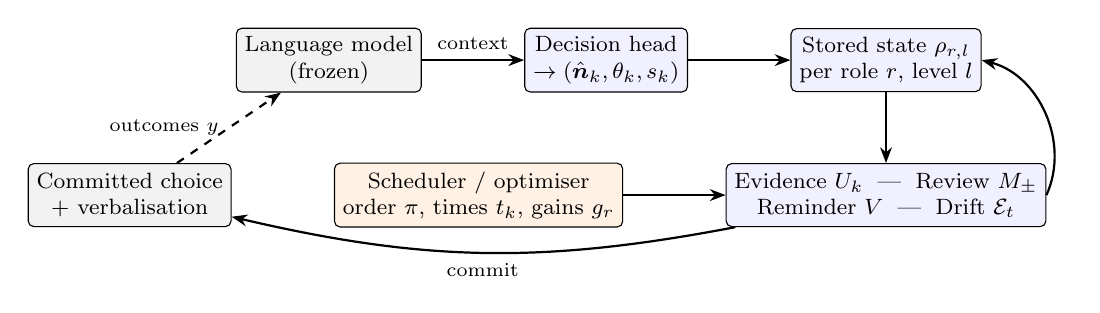
\begin{tikzpicture}[node distance=9mm and 13mm, font=\footnotesize,
  box/.style={draw, rounded corners=2pt, align=center, minimum height=8mm, inner sep=3pt},
  arr/.style={-{Stealth[length=2mm]}, thick}]
\node[box, fill=gray!10] (llm) {Language model\\(frozen)};
\node[box, right=of llm, fill=blue!6] (head) {Decision head\\$\to(\nvec_k,\theta_k,s_k)$};
\node[box, right=of head, fill=blue!6] (state) {Stored state $\rho_{r,l}$\\per role $r$, level $l$};
\node[box, below=of state, fill=blue!6] (ops) {Evidence $U_k$ \;|\; Review $M_\pm$\\Reminder $V$ \;|\; Drift $\mathcal{E}_t$};
\node[box, left=of ops, fill=orange!10] (opt) {Scheduler / optimiser\\order $\pi$, times $t_k$, gains $g_r$};
\node[box, left=of opt, fill=gray!10] (out) {Committed choice\\+ verbalisation};
\draw[arr] (llm) -- node[above]{\scriptsize context} (head);
\draw[arr] (head) -- (state);
\draw[arr] (state) -- (ops);
\draw[arr] (ops.east) to[bend right=50] (state.east);
\draw[arr] (opt) -- (ops);
\draw[arr] (ops) to[bend left=12] node[below]{\scriptsize commit} (out);
\draw[arr, dashed] (out) -- node[left]{\scriptsize outcomes $y$} (llm);
\end{tikzpicture}
\caption{Architecture. The decision layer (blue) stores one state per role and level and applies four kinds of operation. The scheduler (orange) chooses the order, timing, and intensity of operations and the feedback gains. Observed outcomes feed back to the roles (\cref{sec:feedback}).}
\label{fig:framework}
\end{figure}

\subsection{States, roles, and levels}
Each decision has a finite set of options. For role $r$ at level $l\in\{\text{macro},\text{meso},\text{micro}\}$ the state is a density matrix $\rho_{r,l}$ on a $d$-dimensional space $\mathcal{H}_l$. An answer $x$ to question $Q$ is a projector $P_{Q,x}$ with $\sum_x P_{Q,x}=I$; the probability of $x$ is $\tr(P_{Q,x}\rho)$. Following the hierarchy of \citet{li2025narrative}, levels hold different decisions: the macro level holds the goal (pursue the project or not), the meso level the plan (fast-track or phased), and the micro level the concrete action. Because levels live in different spaces, a macro outcome $k$ does not pass its vector down; it \emph{prepares} the meso prior,
\begin{equation}
\rho_{\text{meso}}^{(0)} = W_k\,\rho_{\text{ref}}\,W_k^\dagger ,
\label{eq:prep}
\end{equation}
with $W_k$ a learned unitary per macro outcome. Micro outcomes feed back to the meso state as small rotations (\cref{sec:feedback}), and if the meso probability of reaching the goal falls below a threshold, the macro decision is re-examined. This implements the reflective loop of hierarchical agents \citep{li2025narrative,bougie2026cityreal} without textual memory.

\begin{lemma}[Reciprocity of rank-one answers]
\label{lem:recip}
If the ``yes'' answers to questions $A$ and $B$ are rank-one projectors $P_A=\ket{a}\!\bra{a}$ and $P_B=\ket{b}\!\bra{b}$, then for every state $\rho$ with $\tr(P_A\rho)>0$ and $\tr(P_B\rho)>0$,
\[
P(B_y\,|\,A_y)=P(A_y\,|\,B_y)=|\langle a|b\rangle|^2 .
\]
\end{lemma}
\begin{proof}
After answering $A_y$ the L\"uders state is $P_A\rho P_A/\tr(P_A\rho)=\ket{a}\!\bra{a}$, independent of $\rho$, so $P(B_y|A_y)=\bra{a}P_B\ket{a}=|\langle a|b\rangle|^2$. The same argument with $A$ and $B$ exchanged gives the same value.
\end{proof}

\Cref{lem:recip} is a strong constraint: it holds for pure and mixed states and in any dimension. \Cref{sec:results} shows that published human data violate it, so the ``yes'' and ``no'' answers to realistic questions must be represented by subspaces of rank at least two. This is why the stored state is a density matrix on $d\ge 3$ dimensions rather than a single qubit; the memory cost per decision is $d^2-1$ real numbers.

\subsection{Criterion operators and evidence}
Each role $r$ at level $l$ evaluates a criterion with a Hermitian generator $G_{r,l}$. Evidence of strength $\theta$ about that criterion acts as the unitary
\begin{equation}
U_{r,l}(\theta)=\exp(-i\,\theta\, G_{r,l}/2),\qquad \rho\mapsto U\rho\,U^\dagger .
\label{eq:evidence}
\end{equation}
In the two-dimensional illustration, $G=\nvec\cdot\bsig$ with $\nvec$ a unit vector on the Bloch sphere, so each criterion is a rotation axis. Dynamic models of evidence accumulation in quantum cognition use the same form \citep{busemeyer2006}.

\begin{proposition}[Commuting criteria produce no order effect]
\label{prop:commute}
If $[G_a,G_b]=0$, then $U_aU_b=U_bU_a$ for all evidence strengths, and every outcome probability is independent of the order of the two pieces of evidence. In particular, rotations about a common axis never produce order effects.
\end{proposition}
\begin{proof}
Commuting Hermitian operators have commuting exponentials.
\end{proof}

\begin{proposition}[Role conflict]
\label{prop:comm}
For $G_a=\nvec_a\cdot\bsig$ and $G_b=\nvec_b\cdot\bsig$ with angle $\varphi$ between the axes,
\[
[G_a,G_b]=2i\,(\nvec_a\times\nvec_b)\cdot\bsig,\qquad \big\|[G_a,G_b]\big\|=2\sin\varphi .
\]
\end{proposition}
\begin{proof}
Use $\sigma_j\sigma_k=\delta_{jk}I+i\epsilon_{jkl}\sigma_l$; the operator $\boldsymbol{m}\cdot\bsig$ has eigenvalues $\pm|\boldsymbol{m}|$.
\end{proof}

We call $C_{ab}=\|[G_a,G_b]\|$ the \emph{conflict} between roles $a$ and $b$. It is zero when the criteria are compatible and maximal when their axes are perpendicular. In higher dimensions the same definition applies with the operator norm.

\paragraph{Worked example (corrected).} Our original design evaluated a solar project by rotating about one axis for cost, risk, and timing; by \cref{prop:commute} its outcome could not depend on order. Assigning distinct axes (cost about $y$ with $\theta=-0.3$, risk about $x$ with $\theta=-0.4$, timing about $z$ with $\theta=0.6$, prior polar angle $1.40$) gives the probabilities of approval in \cref{tab:solar}: the same evidence produces approval rates from $0.577$ to $0.720$ depending only on order.

\begin{table}[t]
\centering
\caption{Probability of approval in the solar-project example for all six evaluation orders. Same-axis rotations give identical results in every order (maximum difference $0$ to machine precision).}
\label{tab:solar}
\begin{tabular}{lc}
\toprule
Evaluation order & $P(\text{approve})$\\
\midrule
Risk $\to$ Cost $\to$ Timing & 0.720\\
Cost $\to$ Risk $\to$ Timing & 0.709\\
Risk $\to$ Timing $\to$ Cost & 0.689\\
Cost $\to$ Timing $\to$ Risk & 0.611\\
Timing $\to$ Risk $\to$ Cost & 0.591\\
Timing $\to$ Cost $\to$ Risk & 0.577\\
\bottomrule
\end{tabular}
\end{table}

\subsection{Commitment, review, and reminders}
\emph{Commitment} is a L\"uders projection: answer $x$ occurs with probability $p_x=\tr(P_x\rho)$ and the state becomes $P_x\rho P_x/p_x$. \emph{Review} with intensity $s\in[0,1]$ is an unsharp measurement with Kraus operators
\begin{equation}
M_\pm=\sqrt{\tfrac{1+s}{2}}\,P_x+\sqrt{\tfrac{1-s}{2}}\,(I-P_x),
\label{eq:review}
\end{equation}
which reduces to commitment when $s=1$ and to no disturbance when $s=0$. A \emph{reminder} is a unitary $V(\phi)$ that re-presents a decision's rationale without asking for an answer. The distinction matters because, as \citet{kofman2005} showed for physical decay, coherent modulation can suppress or enhance decay as effectively as measurement while remaining reversible; reminders therefore offer a way to stabilise a decision without locking in the order effects that commitment creates.

\subsection{Drift toward the default}
Between operations, a stored decision interacts weakly with an information environment (news, peer opinion, prices, or task telemetry for an agent). We model this as an open-system channel $\mathcal{E}_t$ that relaxes the state toward a default $\ket{d}$, the status quo. In the simplest, Markovian case this is amplitude damping at rate $\gamma$; \cref{sec:timing} generalises the rate to depend on the environment's spectrum and the review schedule. Each stored state carries a timestamp so that its staleness is part of the memory.

\subsection{One decision cycle, step by step}
\label{sec:cycle}
\Cref{fig:framework2} combines the pieces of this section into one pipeline. A cycle processes one session of new evidence for every role and level:
\begin{enumerate}
\item \textbf{Extract.} A small language model reads the new evidence items and returns, for each, a role, a direction, and a strength. It supplies no probabilities, so the decision layer never reads the model's token distribution. This is the memory's only language-model call before the final answer.
\item \textbf{Rotate.} Each item acts as the unitary $U_{r,l}(\theta)=\exp(-i\theta G_{r,l}/2)$ on the state of its role (\cref{eq:evidence}). Because generators lie on distinct axes, the order of items matters (\cref{prop:commute,prop:comm}). A macro outcome $k$ prepares the meso state through $W_k$ (\cref{eq:prep}), and micro outcomes return as small rotations.
\item \textbf{Review or commit.} A review of intensity $s$ applies $M_\pm$ (\cref{eq:review}); $s=1$ is a L\"uders commitment and $s=0$ leaves the state undisturbed. An optional reminder $V(\varphi)$ re-presents the rationale reversibly, without asking for an answer.
\item \textbf{Drift.} Between operations the state relaxes toward the default $\ket{d}$ at the rate $R$ set by the overlap of the environment spectrum $G(\omega)$ and the review-schedule filter $F_\tau(\omega)$ (\cref{eq:overlap}, panel b). A timestamp records staleness.
\item \textbf{Coordinate.} Role outcomes $y$ are fed back as $u=gy$ (\cref{eq:closed}), which keeps the coordination $I_{ab}$ above the threshold $\theta_c$ (\cref{def:csd}).
\item \textbf{Answer.} When a query arrives, a language model (the same one, or a stronger one) reads only the stored state and verbalises the decision.
\end{enumerate}
Steps 2 to 5 are plain code and use no tokens. The token cost of the memory is therefore the cost of steps 1 and 6, which is why it grows with the amount of new evidence and not with the length of the history.

\begin{figure*}[t]
\centering
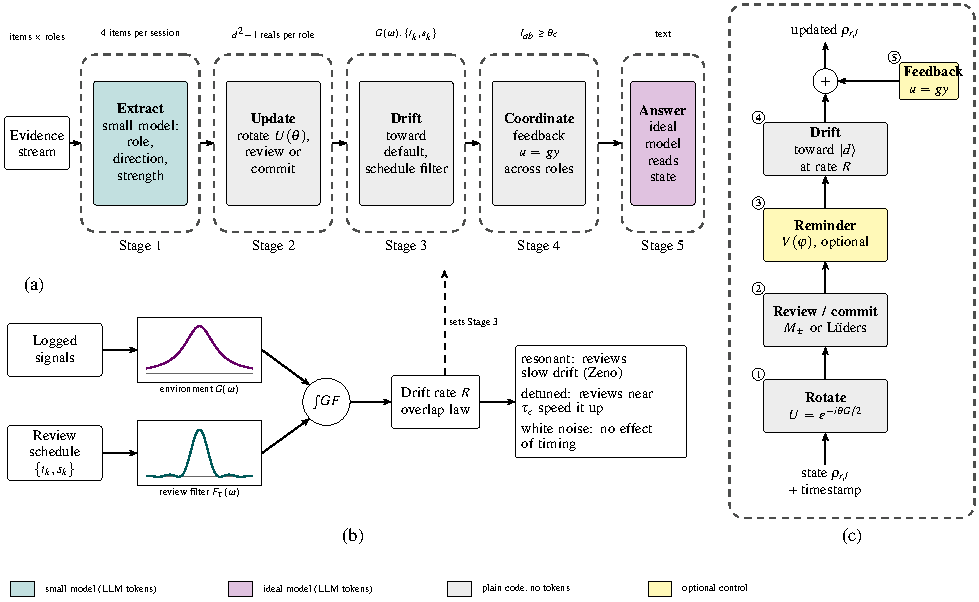
\includegraphics[width=\textwidth]{figs/fig_framework.pdf}
\caption{Step-by-step framework. \textbf{(a)} Pipeline: new evidence is extracted by a small model (Stage 1), applied to the stored state, drifted, and coordinated across roles by code (Stages 2--4), and only then read by an ideal model to answer (Stage 5). \textbf{(b)} Timing mechanism: the spectrum $G(\omega)$ of the logged environment and the filter $F_\tau(\omega)$ of the review schedule overlap to give the drift rate $R$ that sets Stage 3. \textbf{(c)} Update block for one role and level (Stages 2--4): rotation, review or commitment, optional reminder, drift, and cross-role feedback. The extraction, state update, and token accounting are implemented in \texttt{qds\_sim}; the schedule and feedback layers are validated in simulation only; the small-plus-ideal model split is evaluated at pilot scale in \cref{sec:orch}.}
\label{fig:framework2}
\end{figure*}

\section{Timing: review schedules as spectral filters}
\label{sec:timing}

\subsection{The QQ equality and what breaks it}
For two questions answered in sequence with no other operation in between, the QQ equality
\begin{equation}
q \equiv \big[p(A_yB_n)+p(A_nB_y)\big]-\big[p(B_yA_n)+p(B_nA_y)\big] = 0
\label{eq:qq}
\end{equation}
holds for any state and any projectors \citep{wang2013}. The derivation assumes that the only thing changing the state between questions is the first answer. Our framework makes the converse precise: any evidence rotation, reminder, or drift inserted between the questions generically gives $q\neq 0$. For example, with $A=\sigma_z$, $B=\sigma_x$ and prior polar angle $1.40$, inserting a rotation $U_y(0.6)$ between questions gives $q=-0.565$, and inserting amplitude damping with strength $0.3$ gives $q=+0.148$. The size and sign of the violation are thus predictions of the model, not free parameters, once the inserted operation is specified. This extends the explanation of the one failing data set in \citet{wang2013}, where text inserted between questions acted as evidence, to time delays, which act as drift.

Satisfying the equality is not, however, specific to quantum models.

\begin{proposition}[Classical carry-over and the QQ equality]
\label{prop:carry}
Let questions $A$ and $B$, asked first, receive ``yes'' with probabilities $a$ and $b$. Suppose the second answer is pulled toward the first: after a ``yes'' the second question's ``yes'' probability $p$ becomes $p+k_y(1-p)$, and after a ``no'' it becomes $p(1-k_n)$. Then
\[ q=(a-b)(k_n-k_y). \]
In particular, symmetric carry-over ($k_y=k_n$) satisfies the QQ equality exactly while still producing order effects.
\end{proposition}
\begin{proof}
In the $AB$ order the probability of different answers is $a(1-k_y)(1-b)+(1-a)b(1-k_n)$; the $BA$ order exchanges $a$ and $b$. Subtracting gives $(1-k_y)(a-b)+(1-k_n)(b-a)=(a-b)(k_n-k_y)$.
\end{proof}

\Cref{prop:carry} agrees with the observation of \citet{kang2026} that classical repetition mechanisms can satisfy the equality. Passing the $q$-test is therefore necessary but not sufficient evidence for the framework; \cref{sec:design} quantifies how weakly it discriminates.

\subsection{The overlap law}
\citet{kofman2001,kofman2005} considered a state coupled weakly to a continuum and subject to a time-dependent modulation $\epsilon(t)$. Its survival probability is
\begin{equation}
P(t)=\exp\!\big[-R(t)\,Q(t)\big],\qquad R(t)=2\pi\!\int\! d\omega\; G(\omega+\omega_a)\,F_t(\omega),
\label{eq:overlap}
\end{equation}
where $G$ is the coupling spectrum of the reservoir, $F_t(\omega)=|\epsilon_t(\omega)|^2/\!\int|\epsilon_t|^2$ is the normalised spectrum of the modulation over the window $(0,t)$, $\omega_a$ is the transition frequency, and $Q(t)=\int_0^t|\epsilon|^2$ is the fluence. Repeated projective measurement at interval $\tau$ broadens the modulation spectrum to
\begin{equation}
F_\tau(\omega)=\frac{\tau}{2\pi}\,\mathrm{sinc}^2\!\Big(\frac{\omega\tau}{2}\Big),
\label{eq:sinc}
\end{equation}
whose width is about $2\pi/\tau$. If $G$ peaks at $\omega_a$, broadening reduces the overlap (Zeno); if $\omega_a$ lies away from the peak, broadening can increase it (anti-Zeno). Both effects were observed in the same physical system by \citet{fischer2001}.

\paragraph{Decision reading.} We reinterpret the terms of \cref{eq:overlap} for a stored decision. $G(\omega)$ is the spectrum of the information environment, estimated from the autocorrelation of the exogenous signals the decision is exposed to; for an agent these signals are logged, so $G$ can be measured rather than assumed. $\omega_a$ is the decision's characteristic rate, the inverse of the time it would take the evidence dynamics to swing it unaided. $F_t$ is determined by the review schedule $\{(t_k,s_k)\}$ through \cref{eq:review}. $R$ is then the drift rate of the decision toward its default. In this reading the review schedule is a filter designed by the agent or organisation, and the environment spectrum is given.

\begin{proposition}[White-noise null]
\label{prop:null}
If $G(\omega)\equiv G_0$ is constant over the support of $F_t$, then $R(t)=2\pi G_0=\RGR$ for every review schedule.
\end{proposition}
\begin{proof}
$F_t$ is normalised, so $\int G_0F_t\,d\omega=G_0$.
\end{proof}

\Cref{prop:null} is the main falsifiable consequence of the timing layer: review timing can change how fast a decision drifts only if the environment has temporal structure. A memoryless (Markovian Lindblad) drift model, which corresponds to a flat $G$, predicts no such effect. \Cref{sec:results} quantifies the two regimes for a Lorentzian environment with correlation time $\tau_c=1/\xi$.

\paragraph{Two Zeno mechanisms.} The Zeno effect observed by \citet{yearsley2016} arises because measurement interrupts a coherent rotation driven by evidence; it can only slow change. The overlap mechanism arises because measurement reshapes the overlap with a continuum; it can slow or speed change. Our framework contains both, and they make different predictions: the first is monotone in review frequency, the second can be non-monotone. Experiments should be designed to tell them apart (\cref{sec:protocols}).

\section{Feedback: keeping coupled roles coordinated}
\label{sec:feedback}

\subsection{A linear-Gaussian surrogate}
To analyse many coupled roles cheaply, we linearise each state near its default. The two transverse Bloch components of role $r$ form a pair $x_r=(q_r,p_r)$: $q_r$ is the displacement of the commitment and $p_r$ its rate of change. The approximation is crude for a single decision but accurate for a population of agents or respondents, which is the level at which we calibrate. Stacking roles gives
\begin{equation}
dx=A\,x\,dt+B\,dw,\qquad \frac{dV}{dt}=AV+VA^\top+D,
\label{eq:lyap}
\end{equation}
where $V$ is the covariance and $D=BB^\top$. For the hierarchy, $A$ is block lower-triangular (macro drives meso drives micro), mirroring the one-way optical field of \citet{yamamoto2008pra}. Outcomes are observed with noise, $y=Cx+v$ with $\mathbb{E}[dv^2]=(r/\eta)\,dt$, where $\eta\in(0,1]$ is observation efficiency. Following \citet{yamamoto2008pra}, delayed or filtered outcome reporting can be modelled by adding a low-pass filter state.

Proportional feedback $u=g\,y$ applied along directions $f$ gives the closed loop
\begin{equation}
A_{\mathrm{cl}}=A+g\,fC,\qquad D_{\mathrm{cl}}=D+g^2\,\tfrac{r}{\eta}\,ff^\top .
\label{eq:closed}
\end{equation}
The gain reshapes the drift (useful) and injects observation noise in proportion to $g^2$ (harmful). This trade-off is the main lesson we transfer from \citet{yamamoto2008cdc,yamamoto2008pra}.

\subsection{Coordination and its sudden death}
Partition $V=\begin{psmallmatrix}V_1&V_2\\V_2^\top&V_3\end{psmallmatrix}$ for roles $a$ and $b$. We measure coordination by the Gaussian mutual information
\begin{equation}
I_{ab}=\tfrac12\log\frac{\det V_1\,\det V_3}{\det V}
\label{eq:mi}
\end{equation}
and disagreement by $\Delta_{ab}=\mathrm{Var}(q_a-q_b)$.

\begin{definition}[Coordination sudden death]
\label{def:csd}
Given an operational threshold $\theta_c>0$, the minimum coupling at which joint action succeeds, coordination sudden death occurs at the first time $t^\ast$ with $I_{ab}(t^\ast)<\theta_c$.
\end{definition}

The physical phenomenon of entanglement sudden death is a change of topology: entanglement becomes exactly zero in finite time and cannot be recovered by distillation \citep{yamamoto2008pra}. Classical mutual information does not vanish in finite time, so our definition is a threshold crossing. We deliberately avoid logarithmic negativity and other entanglement measures, which require a physical quantum covariance and non-classical correlations that we have no evidence for in cognitive data \citep{dzhafarov2016}.

\section{Optimisation and calibration}
\label{sec:opt}

\subsection{The decision problem}
A static objective of the form $\sum_{r,l}\lambda_l w_{r,l}\tr(G_{r,l}\rho)$ equals $\tr(H\rho)$ for a single Hermitian $H$ and therefore cannot depend on order. Order and timing enter only through the sequence of operations, so the objective must be defined over that sequence. Let $P_l^{\mathrm{goal}}$ be the projector onto the goal subspace at level $l$. The decision variables are the review order $\pi$, review times $\{t_k\}$, intensities $\{s_k\}$, reminder phases $\{\phi_k\}$, and feedback gains $\{g_r\}$. We solve
\begin{align}
\max_{\pi,\{t_k,s_k,\phi_k\},\{g_r\}}\quad & \sum_l \lambda_l\,\tr\!\big(P_l^{\mathrm{goal}}\rho_l(T)\big)\;-\;c_{\mathrm{rev}}\sum_k s_k^2\;-\;c_{\mathrm{rem}}\sum_k|\phi_k| \label{eq:obj}\\
\text{s.t.}\quad & P(\text{risk}=\text{bad})\le\varepsilon, \tag{hard risk gate}\\
& P_{\mathrm{stay}}(T)\ge F_{\min}\ \text{for committed decisions}, \tag{stability}\\
& I_{ab}(t)\ge\theta_c\ \ \forall t\in[0,T],\ \forall\ \text{coupled}\ (a,b), \tag{no coordination death}\\
& A_{\mathrm{cl}}\ \text{Hurwitz},\qquad \textstyle\sum_k \mathrm{cost}(s_k)\le B. \tag{stability, budget}
\end{align}
The hard risk gate follows the reviewer protocol of \citet{ye2026agonalpha}, in which only verified failures veto an outcome and all other findings are advisory. A second, robustness-oriented objective replaces the first term by the order sensitivity $S=\max_\pi P-\min_\pi P$ to be minimised, which is appropriate when the goal is a fair review process rather than a favourable one.

\begin{algorithm}[t]
\caption{Schedule and order optimisation}
\label{alg:opt}
\begin{algorithmic}[1]
\Require calibrated parameters $\Theta$, environment spectrum $G$, horizon $T$, budget $B$
\For{each candidate order $\pi$ (enumerate if $n\le 5$, else beam search or MCTS)}
  \State initialise schedule $\{t_k,s_k,\phi_k\}$
  \Repeat
    \State simulate $\rho_l(T)$ by composing $U$, $M_\pm$, $V$, and $\mathcal{E}$ in order
    \State evaluate objective \eqref{eq:obj}; use \eqref{eq:overlap} as a fast surrogate for drift
    \State gradient step on continuous variables (differentiable simulator)
  \Until{converged}
  \State solve $A_{\mathrm{cl}}V+VA_{\mathrm{cl}}^\top+D_{\mathrm{cl}}=0$ for gains $g$; check constraints
\EndFor
\State \Return best feasible $(\pi,\{t_k,s_k,\phi_k\},\{g_r\})$
\end{algorithmic}
\end{algorithm}

\subsection{Calibration}
The parameters are the criterion generators and evidence strengths, the preparation unitaries $W_k$, feedback gains, the environment spectrum $(G,\omega_a)$, review sharpness $s$ for each elicitation format, and observation efficiency $\eta$. We fit them by maximum likelihood or hierarchical Bayes on sequential response data. The loss is a proper scoring rule \citep{gneiting2007}, primarily the logarithmic score and secondarily the Brier score. Following \citet{drissi2025}, the natural-gradient (Fisher) metric is matched to the logarithmic score; for the Brier score we use the metric induced by its divergence.

Two design choices make the fit informative rather than merely flexible. First, following \citet{yearsley2016}, evidence parameters are fitted on conditions without intermediate reviews, and schedule effects are then \emph{predicted} without further fitting. Second, for agents, $G$ is estimated directly from the periodogram of logged environmental signals. For population-level calibration across many agents we adopt the objective of \citet{bougie2026cityreal}: a geometric mean of normalised discrepancies, here on outcome distributions, order effects, and per-role and per-level statistics, multiplied by penalties against loss of individual plausibility and of population diversity. Model comparison uses cross-validated log score, and parameter recovery is checked on simulated data before fitting real data.

\section{Results}
\label{sec:results}

All simulation results are produced by an open Python package (\texttt{qds\_sim}) with fixed random seeds; a test suite of 13 checks covers \cref{prop:commute,prop:comm,prop:carry,prop:null}, \cref{lem:recip}, and the published values reproduced below. The simulation experiments run in about seven minutes on a laptop; the token benchmark of \cref{sec:tokens} additionally needs API access.

\subsection{Reanalysis of six published order-effect data sets}
We reanalysed the six data sets reported by \citet{wang2013}: four national Gallup split-ballot surveys reviewed by \citet{moore2002} and two laboratory replications. For each we computed the $q$ statistic and its $z$-test, and fitted four models by maximum likelihood to the eight response-sequence frequencies: (a) an \emph{order-free} classical model with one joint distribution shared by both orders (3 free parameters); (b) the \emph{QQ-constrained} model, which leaves the sequence probabilities free except for the equality \eqref{eq:qq} (5 parameters); (c) a quantum model in three dimensions with \emph{rank-one} ``yes'' projectors (4 parameters); and (d) the saturated model (6 parameters). \Cref{tab:qq} reports the results.

\begin{table}[t]
\centering
\caption{Reanalysis of the six data sets in \citet{wang2013}. $q$ and $z$: QQ test (sign convention $p_{AB}-p_{BA}$). $G^2$: likelihood-ratio deviance from the saturated model for the order-free classical model (df $=3$), the QQ-constrained model (df $=1$), and the rank-one quantum model (df $=2$). Last two columns: empirical $P(B_y|A_y)$ in the $AB$ order versus $P(A_y|B_y)$ in the $BA$ order, which \cref{lem:recip} requires to be equal; and the model with lowest AIC.}
\label{tab:qq}
\small
\begin{tabular}{lcrrrrrcl}
\toprule
Data set & $N_{AB}/N_{BA}$ & $q$ & $z$ & $G^2_{\text{free}}$ & $G^2_{\text{QQ}}$ & $G^2_{\text{rank-1}}$ & $P(B|A)$ / $P(A|B)$ & Best AIC\\
\midrule
Clinton--Gore & 447/432 & -0.003 & -0.11 & 10.1 & 0.01 & 104 & 0.92 / 0.74 & QQ-constr.\\
Gingrich--Dole & 437/377 & -0.003 & -0.09 & 4.4 & 0.01 & 235 & 0.83 / 0.50 & QQ-constr.\\
White--Black & 459/486 & -0.019 & -0.75 & 73.0 & 0.56 & 188 & 0.96 / 0.87 & QQ-constr.\\
Rose--Jackson & 506/462 & +0.151 & +5.30 & 67.2 & 28.56 & 106 & 0.51 / 0.86 & Saturated\\
Racial hostility (lab) & 116/108 & +0.076 & +1.22 & 28.7 & 1.48 & 62 & 0.81 / 0.83 & QQ-constr.\\
Affirmative action (lab) & 118/106 & +0.043 & +0.83 & 1.7 & 0.69 & 26 & 0.92 / 0.81 & Order-free\\
\bottomrule
\end{tabular}
\end{table}

Three findings stand out. First, the $q$ and $z$ values agree with those published by \citet{wang2013} to within $0.01$, and the QQ-constrained deviance for the Rose--Jackson data, $G^2=28.56$, reproduces their reported $28.57$. Only that data set, in which background text was read between questions, violates the equality ($z=5.30$). Second, the QQ-constrained model has the lowest AIC in four of the six data sets; the saturated model wins for Rose--Jackson, as the theory predicts, and the order-free classical model wins for the affirmative-action data, where order effects are small. Third, the rank-one quantum model is rejected in every data set ($G^2\ge 26$ on 2 df, $p<10^{-5}$). The reason is visible in the last columns: the reciprocity required by \cref{lem:recip} is violated by large margins, for example $0.83$ versus $0.50$ for Gingrich--Dole and $0.51$ versus $0.86$ for Rose--Jackson. Answer subspaces for realistic questions must therefore have rank of at least two, a design constraint that our original single-qubit proposal did not meet.

\subsection{Order sensitivity tracks role conflict}
We applied two rotations of equal strength ($\theta=1$) about axes separated by angle $\varphi$ (both axes in the $x$--$y$ plane, with the outcome measured along $z$) to 2{,}000 random pure states for each of 37 values of $\varphi\in[0,\pi]$, and recorded the mean absolute difference in $P(\mathrm{yes})$ between the two orders. \Cref{fig:order} shows that order sensitivity is zero at $\varphi=0$ and $\varphi=\pi$, where the generators commute, and rises with the conflict $C_{ab}=2\sin\varphi$ of \cref{prop:comm}; across the sweep the Pearson correlation between the two is $r=0.86$, and the maximum mean order sensitivity is $0.15$. The value of $r$ depends on this geometry (a different choice of measured axis gives a different curve with the same zeros), so the setup is part of the result. The conflict metric is therefore a usable, closed-form predictor of how much the order of two roles' reviews will matter.

\begin{figure}[t]
\centering
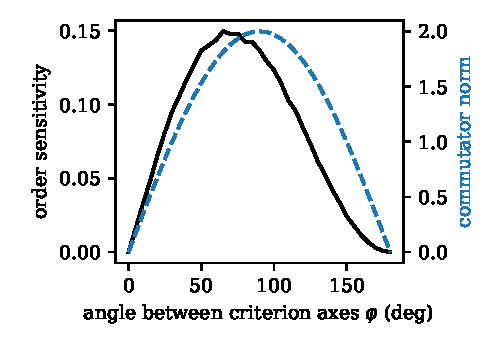
\includegraphics[width=0.48\linewidth]{figs/order_vs_angle.pdf}\hfill
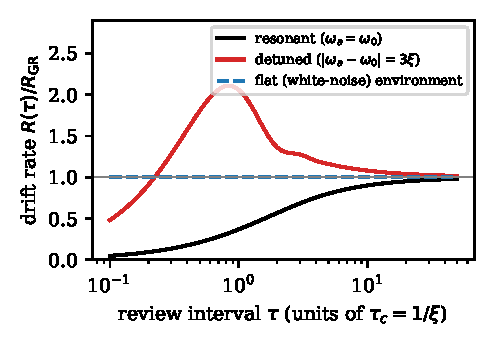
\includegraphics[width=0.48\linewidth]{figs/zeno_antizeno.pdf}
\caption{\textbf{Left:} mean order sensitivity over 2{,}000 random states (solid, left axis) and commutator norm $2\sin\varphi$ (dashed, right axis) as functions of the angle between two criterion axes. \textbf{Right:} drift rate under periodic projective review, relative to the unreviewed (golden-rule) rate, for a Lorentzian environment with correlation time $\tau_c$. Resonant decision: reviews always slow drift (decision Zeno). Detuned decision: reviews near $\tau\approx\tau_c$ accelerate drift (decision anti-Zeno). White-noise environment: no schedule effect (\cref{prop:null}).}
\label{fig:order}
\end{figure}

\subsection{Decision Zeno and anti-Zeno regimes}
We evaluated \cref{eq:overlap,eq:sinc} numerically for a Lorentzian environment $G(\omega)=\frac{\Gamma}{2\pi}\xi^2/[(\omega-\omega_0)^2+\xi^2]$ with $\xi=1$ (so $\tau_c=1$) and review intervals $\tau\in[0.1,50]\,\tau_c$ (\cref{fig:order}, right). For a decision resonant with the environment ($\omega_a=\omega_0$), review always slows drift: the rate falls to $0.05\,\RGR$ at $\tau=0.1\,\tau_c$ and approaches $\RGR$ only for $\tau\gg\tau_c$. For a detuned decision ($|\omega_a-\omega_0|=3\xi$), review at short intervals still slows drift ($0.48\,\RGR$ at $\tau=0.1\,\tau_c$), but review at $\tau\approx 0.84\,\tau_c$ more than doubles it ($2.11\,\RGR$). For a flat environment the rate equals $\RGR$ for every interval to within $0.2\%$ numerical error, as \cref{prop:null} requires.

The cognitive reading is a concrete prediction. Re-examining a decision whose natural rate is out of step with the dominant pressure in its environment, at intervals comparable to that pressure's timescale, exposes the decision to that pressure and speeds its abandonment. Reviewing a decision more often is therefore not always stabilising.

\subsection{Feedback preserves coordination}
We simulated two roles with identical damped dynamics ($\gamma=0.5$, natural frequency $1$), no direct coupling, observation of the disagreement $q_2-q_1$ with noise $r=0.25$, and feedback that moves the roles toward each other. \Cref{fig:feedback} (left) shows the steady-state disagreement as a function of gain. Without feedback it is $2.0$. With efficient observation ($\eta=1$) the optimum gain $g^\ast=1.14$ reduces it to $0.54$ ($-73\%$); at $\eta=0.5$, $g^\ast=0.76$ gives $0.73$ ($-64\%$); at $\eta=0.2$, $g^\ast=0.43$ gives $1.03$ ($-49\%$). An Euler--Maruyama simulation of the closed loop agrees with the analytic covariance to within 6\%. Beyond the optimum, noise injected by the $g^2$ term in \cref{eq:closed} dominates. The optimal gain falls as observation degrades, but feedback helps at every efficiency tested, mirroring the robustness to detector loss reported by \citet{yamamoto2008pra}.

\Cref{fig:feedback} (right) starts the two roles in strong agreement (correlation $0.95$) and tracks their mutual information. Without feedback, coordination falls below the threshold $\theta_c=0.2$ nats at $t^\ast=1.61$ and decays toward zero. With feedback ($g=0.6$) it never crosses the threshold and settles at $0.25$ nats.

\begin{figure}[t]
\centering
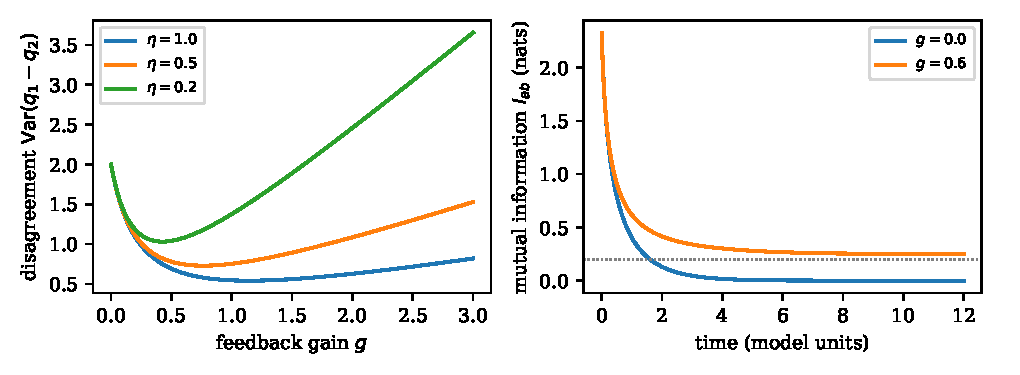
\includegraphics[width=0.92\linewidth]{figs/feedback.pdf}
\caption{\textbf{Left:} steady-state disagreement between two roles versus feedback gain, for three observation efficiencies; each curve has an interior optimum. \textbf{Right:} mutual information from an initially agreed state without feedback (crosses the threshold, dotted, at $t^\ast=1.61$) and with feedback (stays above it).}
\label{fig:feedback}
\end{figure}

\subsection{Simulation-based design analysis}
\label{sec:design}
Before collecting new data, we simulated each proposed study (\cref{sec:protocols}) with synthetic participants generated from the models. These simulations do not test the hypotheses; they check that the planned analyses recover what generated the data, estimate effect sizes, and set sample sizes.

\paragraph{H1: two-stage prediction.} Simulated participants read 12 pieces of weak evidence (each piece a rotation by $\delta$, drawn per participant from a normal distribution with mean $0.13$ and standard deviation $0.03$) and made 0, 1, 2, 3, 5, or 11 intermediate judgments ($n=600$ per group). The probability of a final ``guilty'' judgment fell from $0.47$ with no intermediate judgments to $0.26$, $0.19$, $0.16$, $0.13$, and $0.09$; a Bayesian baseline calibrated to the same no-judgment group stayed flat. Fitting $\delta$ on the no-judgment group alone gave $\hat\delta=0.125$, and predictions for the other five groups had root-mean-square error $0.005$. One caveat matters for real data: because the no-judgment prediction $\sin^2(6\delta)$ is periodic in $\delta$, a single group identifies $\delta$ only on the monotone branch $12\delta\le\pi$, an assumption that must be stated.

\paragraph{H2: schedule effects.} Participants held a committed decision for $T=20\,\tau_c$, with the environment scaled so that about half retained it without review ($n=800$ per cell). For detuned decisions in an autocorrelated environment, retention fell from $0.50$ without review to $0.23$ with reviews at $\tau\approx0.84\,\tau_c$ (anti-Zeno) and rose to $0.73$ with reviews at $\tau=0.1\,\tau_c$ (Zeno). Resonant decisions showed only the Zeno effect, with retention up to $0.97$. In the white-noise environment retention stayed between $0.47$ and $0.51$ for every schedule, as \cref{prop:null} requires (\cref{fig:design}, top).

\paragraph{H3: reminders versus recommitment.} A committed decision was perturbed by transverse pressure that was redrawn at rate $\nu$ and by weak drift toward the default, with a budget of $K$ interventions ($n=1{,}000$ per cell). When the pressure changed slowly ($\nu=0$, $K=4$), reminders implemented as coherent refocusing retained the decision with probability $0.75$, against $0.57$ for forced recommitment and $0.46$ with no intervention; recommitment also left larger order effects in a later pair of questions ($0.17$ versus $0.10$). When the pressure fluctuated quickly ($\nu=8$), the advantage of reminders disappeared ($0.68$ versus $0.66$ at $K=4$). This is the boundary predicted by \citet{kofman2005}: coherent control helps only when it is faster than the environment's correlation time.

\paragraph{H4: power.} Across 600 random four-dimensional models, drift alone between two questions produced median $|q|=0.04$ when half the state had drifted and $0.08$ at near-complete drift, with a long tail (90th percentile $0.22$) and some models near zero. Intervening content produced $q\approx0.14$; with 250 participants per order the $q$-test detected it with probability $0.97$ for back-to-back questions and $0.91$ after a one-hour delay, and with 100 per order only $0.65$ and $0.51$. The false-positive rate under the null stayed near $0.05$ for every sample size.

\paragraph{Model recovery.} We generated split-ballot data from four processes, namely a quantum model with rank-two answer subspaces in four dimensions, an order-free classical model, symmetric carry-over, and asymmetric carry-over (\cref{prop:carry}), and classified each data set by lowest AIC (300 data sets per cell). Quantum data were assigned to the QQ-constrained model in 75\%, 78\%, and 84\% of cases at 200, 500, and 1{,}000 participants per order, and order-free data to the order-free model in 81--87\%. Symmetric carry-over was assigned to the QQ-constrained model in up to 62\% of cases and was rejected by the $q$-test at the nominal 5\% rate, as \cref{prop:carry} implies; asymmetric carry-over was rejected in only 38\% of cases even at 1{,}000 per order (\cref{fig:design}, bottom). Order-effect data alone therefore discriminate weakly between quantum and classical accounts, which is why the framework must be tested on the joint pattern of H1--H5.

\begin{figure}[t]
\centering
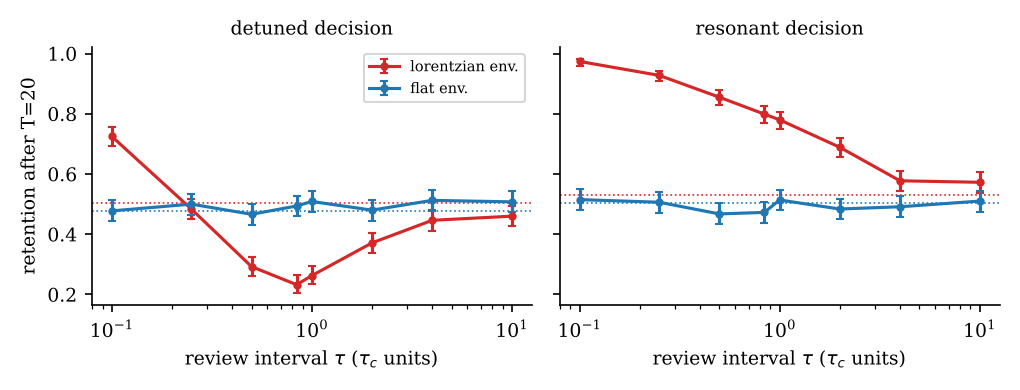
\includegraphics[width=0.98\linewidth]{figs/fig_h2_schedule.png}\\[4pt]
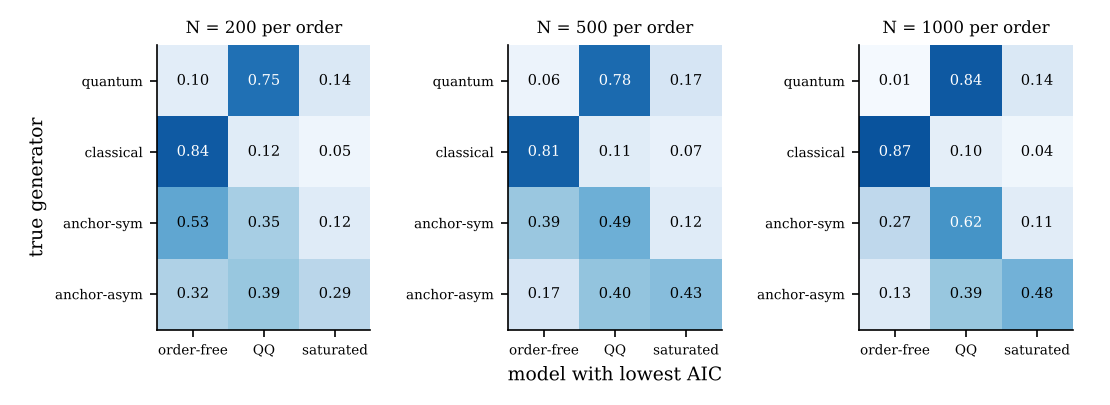
\includegraphics[width=0.98\linewidth]{figs/fig_confusion.png}
\caption{Simulation-based design analysis (synthetic data). \textbf{Top:} retention of a committed decision after $T=20\,\tau_c$ versus review interval (H2). \textbf{Bottom:} model-recovery confusion matrices at 200, 500, and 1{,}000 participants per order: the fraction of data sets from each generating process assigned to each fitted model by AIC.}
\label{fig:design}
\end{figure}

\subsection{Agent memory: token benchmark}
\label{sec:tokens}
\paragraph{Mock harness.} For Study 3 we first built a harness in which three roles feed templated evidence to an agent over ten sessions and four memory schemes store it. With a mock language model, the transcript memory grew to about 425 tokens per project, a six-item summary to about 64 tokens, and the classical belief and quantum states used 2 and 4 numbers. Only the quantum memory produced question-order effects (mean $|\Delta P|=0.16$). These are storage footprints that follow from the construction of each scheme; they are not API costs and are reported only to show that the pipeline works.

\paragraph{Real-model benchmark.} \Cref{fig:arch} shows the three memory architectures compared. We ran the harness with \texttt{claude-haiku-5-5} (extended thinking disabled) and recorded the token counts reported by the API for every call. Five memories see identical evidence: the full transcript, a rolling summary, retrieval of the most relevant items, the decision state (the model extracts a role, direction, and strength for each evidence item, and the state is updated outside the model), and the state followed by a verbalising call. Decision quality is scored against a synthetic ground truth: approve if and only if the equal-weight sum of signed evidence strengths is positive. Evidence extraction was batched per session; no run had parse errors, truncated replies, or empty replies. (A first one-project pilot produced 15 parse errors, which were resolved (extended thinking disabled) before the main runs; the pilot is excluded from the tables.)

\begin{figure}[!t]
\centering
\resizebox{\linewidth}{!}{%
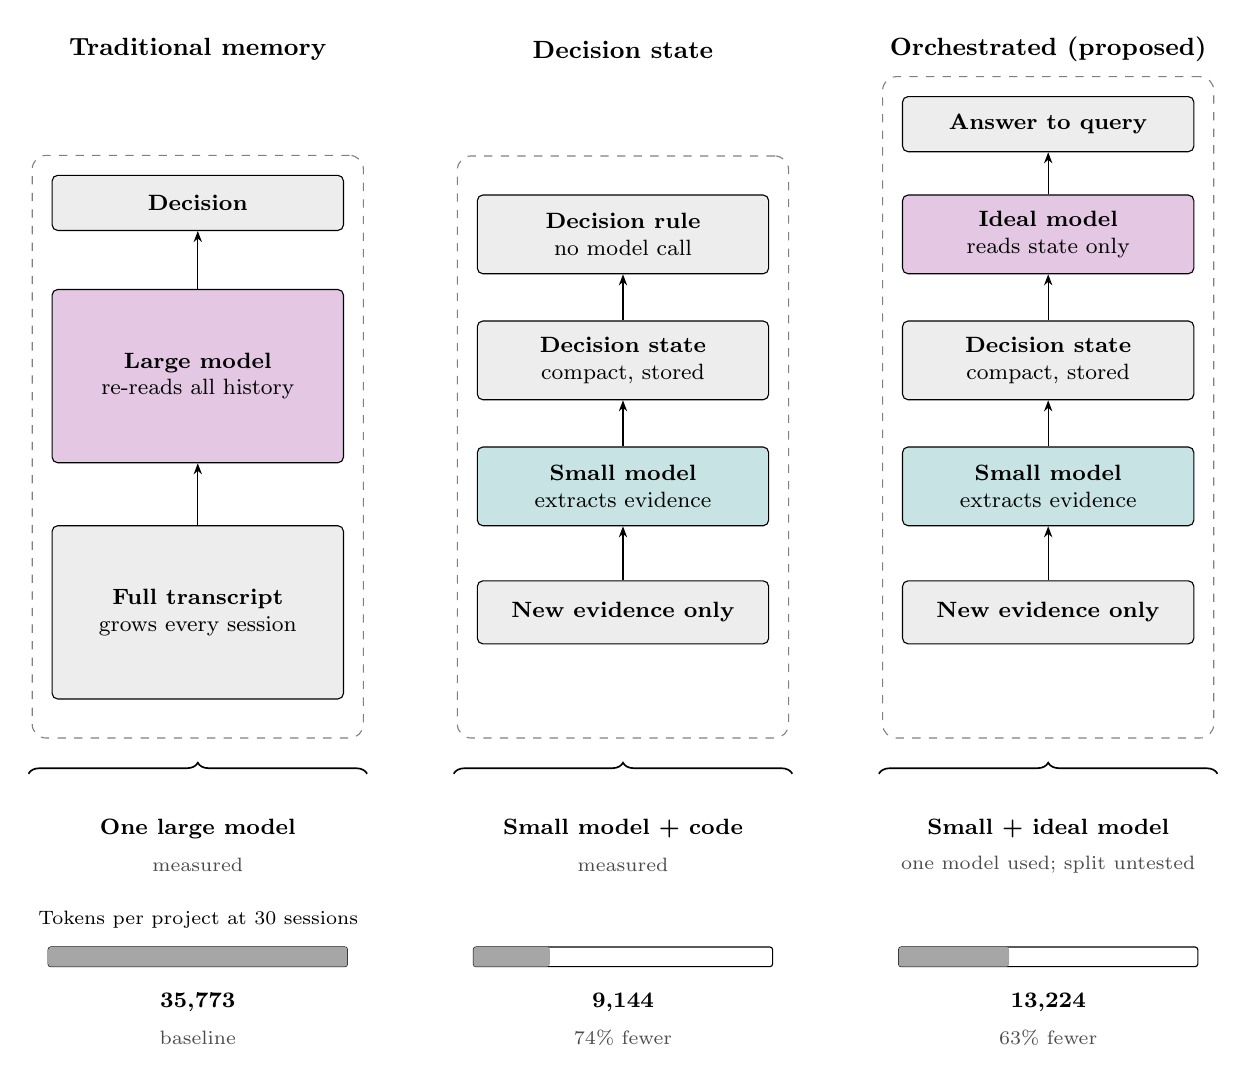
\begin{tikzpicture}[
  font=\footnotesize,
  blk/.style={draw, rounded corners=2pt, minimum width=3.7cm, align=center, inner sep=3pt, line width=0.4pt},
  gry/.style={blk, fill=gray!14},
  sml/.style={blk, fill=teal!22},
  lrg/.style={blk, fill=violet!22},
  arr/.style={-{Stealth[length=4pt]}, line width=0.5pt},
  pan/.style={draw=gray, dashed, rounded corners=5pt, inner sep=7pt, line width=0.4pt},
  brc/.style={decorate, decoration={brace, mirror, amplitude=4pt}, line width=0.6pt}
]
% Panel A: traditional transcript memory
\node[gry, minimum height=2.2cm] (a1) at (0,0) {\textbf{Full transcript}\\grows every session};
\node[lrg, minimum height=2.2cm] (a2) at (0,3.0) {\textbf{Large model}\\re-reads all history};
\node[gry, minimum height=0.7cm] (a3) at (0,5.2) {\textbf{Decision}};
\draw[arr] (a1.north) -- (a2.south);
\draw[arr] (a2.north) -- (a3.south);
\coordinate (aB) at (0,-1.35);
\node[pan, fit=(a3)(aB)(a1)] (pA) {};
\node[font=\small\bfseries] at (0,7.15) {Traditional memory};
% Panel B: decision state, small model + code
\node[gry, minimum height=0.8cm] (b1) at (5.4,0) {\textbf{New evidence only}};
\node[sml, minimum height=1.0cm] (b2) at (5.4,1.6) {\textbf{Small model}\\extracts evidence};
\node[gry, minimum height=1.0cm] (b3) at (5.4,3.2) {\textbf{Decision state}\\compact, stored};
\node[gry, minimum height=1.0cm] (b4) at (5.4,4.8) {\textbf{Decision rule}\\no model call};
\draw[arr] (b1.north) -- (b2.south);
\draw[arr] (b2.north) -- (b3.south);
\draw[arr] (b3.north) -- (b4.south);
\coordinate (bB) at (5.4,-1.35); \coordinate (bT) at (5.4,5.55);
\node[pan, fit=(bT)(bB)(b1)] (pB) {};
\node[font=\small\bfseries] at (5.4,7.15) {Decision state};
% Panel C: orchestrated, small + ideal model
\node[gry, minimum height=0.8cm] (c1) at (10.8,0) {\textbf{New evidence only}};
\node[sml, minimum height=1.0cm] (c2) at (10.8,1.6) {\textbf{Small model}\\extracts evidence};
\node[gry, minimum height=1.0cm] (c3) at (10.8,3.2) {\textbf{Decision state}\\compact, stored};
\node[lrg, minimum height=1.0cm] (c4) at (10.8,4.8) {\textbf{Ideal model}\\reads state only};
\node[gry, minimum height=0.7cm] (c5) at (10.8,6.2) {\textbf{Answer to query}};
\draw[arr] (c1.north) -- (c2.south);
\draw[arr] (c2.north) -- (c3.south);
\draw[arr] (c3.north) -- (c4.south);
\draw[arr] (c4.north) -- (c5.south);
\coordinate (cB) at (10.8,-1.35);
\node[pan, fit=(c5)(cB)(c1)] (pC) {};
\node[font=\small\bfseries] at (10.8,7.15) {Orchestrated (proposed)};
% braces and labels
\foreach \x/\t/\u in {0/{One large model}/{measured}, 5.4/{Small model + code}/{measured}, 10.8/{Small + ideal model}/{one model used; split untested}} {
  \draw[brc] (\x+2.15,-2.05) -- (\x-2.15,-2.05);
  \node[font=\footnotesize\bfseries] at (\x,-2.75) {\t};
  \node[font=\scriptsize, text=black!70] at (\x,-3.2) {\u};
}
% token bars
\node[font=\scriptsize, anchor=west] at (-2.15,-3.9) {Tokens per project at 30 sessions};
\foreach \x/\w/\n/\r in {0/3.8/{35,773}/{baseline}, 5.4/0.971/{9,144}/{74\% fewer}, 10.8/1.404/{13,224}/{63\% fewer}} {
  \draw[line width=0.4pt, rounded corners=1pt] (\x-1.9,-4.25) rectangle (\x+1.9,-4.5);
  \fill[gray!70, rounded corners=1pt] (\x-1.9,-4.25) rectangle (\x-1.9+\w,-4.5);
  \node[font=\footnotesize\bfseries] at (\x,-4.95) {\n};
  \node[font=\scriptsize, text=black!70] at (\x,-5.4) {\r};
}
\end{tikzpicture}}
\caption{Memory architectures compared in the token benchmark. \textbf{Left:} a large model re-reads the full transcript at every session. \textbf{Middle:} a small model turns each session's new evidence into role, direction, and strength, a stored decision state is updated in code, and the decision needs no further model call. \textbf{Right:} a proposed orchestration in which an ideal model reads only the compact state to write the answer. Bars show tokens per project at 30 sessions (\cref{tab:tokens}) relative to the transcript. The right-hand value (13,224 tokens) was measured with a single model performing both steps; the small-plus-ideal split is evaluated at pilot scale in \cref{sec:orch}.}
\label{fig:arch}
\end{figure}

\begin{table}[t]
\centering
\caption{Token benchmark with a real language model (\texttt{claude-haiku-5-5}; API-reported tokens). Tokens are totals per project; ratio is relative to the transcript memory. Accuracy is against the synthetic ground truth with a 95\% normal-approximation interval; agreement is the fraction of projects where the final decision equals the transcript's.}
\label{tab:tokens}
\small
\begin{tabular}{llrrcccc}
\toprule
Run & Memory & Tokens & Ratio & Accuracy [95\% CI] & Brier & Agree\\
\midrule
\multirow{5}{*}{\shortstack[l]{10 sessions\\$n=30$ projects}}
 & Transcript & 4{,}886 & 1.00 & 0.73 [0.58, 0.89] & 0.217 & 1.00\\
 & Summary & 7{,}455 & 1.53 & 0.53 [0.35, 0.71] & 0.258 & 0.67\\
 & Retrieval & 2{,}038 & 0.42 & 0.43 [0.26, 0.61] & 0.285 & 0.57\\
 & State & 3{,}049 & 0.62 & 0.47 [0.29, 0.65] & 0.328 & 0.40\\
 & State + verbalise & 4{,}413 & 0.90 & 0.47 [0.29, 0.65] & 0.325 & 0.40\\
\midrule
\multirow{5}{*}{\shortstack[l]{30 sessions\\$n=15$ projects}}
 & Transcript & 35{,}773 & 1.00 & 0.40 [0.15, 0.65] & 0.295 & 1.00\\
 & Summary & 23{,}119 & 0.65 & 0.40 [0.15, 0.65] & 0.332 & 0.73\\
 & Retrieval & 6{,}224 & 0.17 & 0.33 [0.09, 0.57] & 0.318 & 0.67\\
 & State & 9{,}144 & 0.26 & 0.53 [0.28, 0.79] & 0.291 & 0.33\\
 & State + verbalise & 13{,}224 & 0.37 & 0.53 [0.28, 0.79] & 0.297 & 0.33\\
\bottomrule
\end{tabular}
\end{table}

\Cref{tab:tokens} gives the results. The state memory used 38\% fewer tokens than the transcript at 10 sessions and 74\% fewer at 30, because the transcript is re-read at every session and its cost grows faster than linearly with history, whereas the state's cost grows roughly linearly. Four limits apply. First, retrieval was cheaper than the state memory at both history lengths ($-58\%$ and $-83\%$ against the transcript). Second, decision quality does not support a claim of parity: at 10 sessions the state's accuracy of $0.47$ lies below the transcript's $0.73$ (the intervals barely overlap), and the state's final decision agreed with the transcript's in only 40\% of projects; at 30 sessions all accuracies are within sampling error ($n=15$). Third, most of the state's tokens are output tokens from the extraction call (31{,}590 of 91{,}463 at 10 sessions), so the saving is not the four-number storage footprint of the mock harness; without batching, extraction repeats its instructions at every call and the state memory used 1.31 times the transcript's tokens at 10 sessions (6{,}395 versus 4{,}863 per project, 15 projects). Fourth, the extraction itself is imperfect: on 1{,}200 items the model recovered the evidence direction correctly 82\% of the time, with a mean absolute error of 0.30 in strength, which limits any state built from it; \cref{sec:noise} shows, however, that the state's own functional form is the larger limit. The ground truth is additive and therefore favours additive memories, evidence is templated, and the numbers of projects are small.

\paragraph{Orchestration with a small and an ideal model.} The right-hand panel of \cref{fig:arch} uses a small model only to extract evidence and a stronger model only to read the compact state and answer. The single-model run above bounds only the token cost of the extra call; the split itself is evaluated in \cref{sec:orch}.

\paragraph{Exploratory rescaling.} Rerunning the 10-session condition with the state's evidence strength scaled by $0.1$ (same extraction cost, 3{,}045 tokens per project) gave accuracy $0.63$ [0.46, 0.81], Brier $0.208$, and agreement $0.83$ with the transcript, against $0.67$ and $0.226$ for the transcript in that run. This scale was chosen after seeing the unscaled results on the same 30 projects, so it is an exploratory, tuned result and not evidence (\cref{sec:noise} explains why small rotations help: they nearly commute, so the state approximates an additive rule); it must be confirmed on fresh projects with the scale fixed in advance. The corresponding 30-session rerun has not been run.

\begin{figure}[t]
\centering
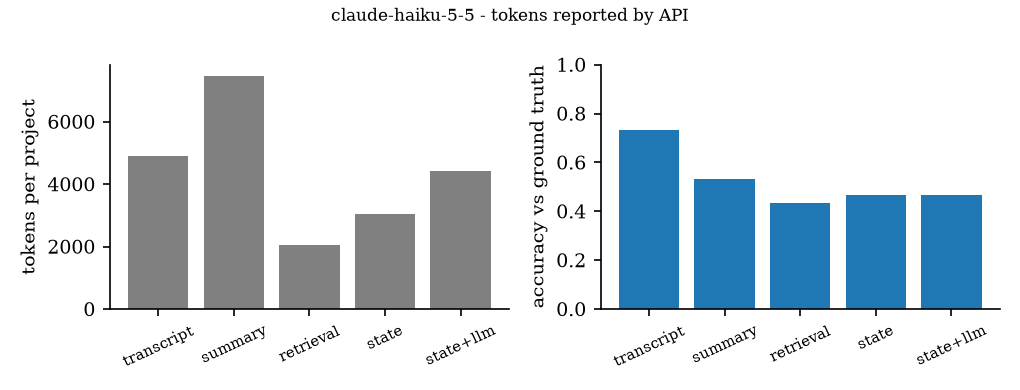
\includegraphics[width=0.98\linewidth]{figs/fig_tokens_s10.png}\\[4pt]
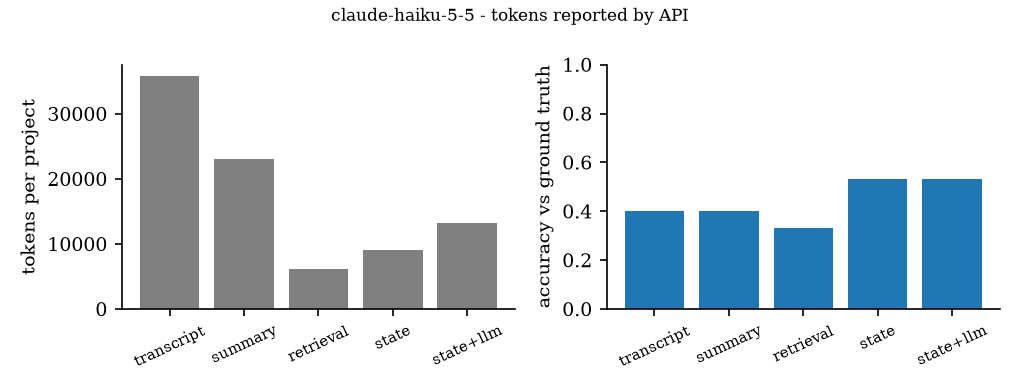
\includegraphics[width=0.98\linewidth]{figs/fig_tokens_s30.png}
\caption{Token benchmark with \texttt{claude-haiku-5-5}: tokens per project and accuracy against the synthetic ground truth for each memory, at 10 sessions ($n=30$ projects, top) and 30 sessions ($n=15$, bottom).}
\label{fig:tokens}
\end{figure}

\subsection{Orchestration benchmark: small extractor, ideal answerer}
\label{sec:orch}
We implemented the pipeline of \cref{fig:framework2} (\texttt{qds\_sim} experiment e8) with \texttt{claude-haiku-5-5} as the small model and \texttt{claude-sonnet-5-5} as the ideal model, and compared five schemes on identical evidence: the ideal model re-reading the transcript (\emph{transcript-ideal}, the baseline), the small model re-reading it (\emph{transcript-small}), retrieval of the latest items with the small model, the state with the decision read from it in code (\emph{state-code}, small-model extraction only), and the orchestrated pipeline (small-model extraction, state, ideal model answering from a one-line state description). Scoring is as in \cref{sec:tokens}. Dollar figures assume prices of \$1 and \$5 (small model) and \$3 and \$15 (ideal model) per million input and output tokens; these are illustrative placeholders, not list prices, so the cost columns should be read as ratios under that assumption. We ran 10 projects of 10 sessions (500 calls), 5 projects of 30 sessions (750 calls), and 5 projects of 30 sessions with an answer only every fifth session (270 calls); all three runs had no parse errors, truncated replies, or empty replies.

\begin{table}[t]
\centering
\caption{Orchestration benchmark with real models (token counts reported by the API; prices are assumptions, see text). Tokens and cost are per project; accuracy has a 95\% Wilson interval. In the last block an answer is given only every fifth session; extraction still runs every session.}
\label{tab:orch}
\small
\begin{tabular}{llrrcc}
\toprule
Run & Scheme & Tokens & Cost (\$) & Accuracy [95\% CI] & Brier\\
\midrule
\multirow{5}{*}{\shortstack[l]{10 sessions\\$n=10$}}
 & Transcript, ideal & 7{,}407 & 0.054 & 0.90 [0.60, 0.98] & 0.138\\
 & Transcript, small & 4{,}873 & 0.005 & 0.80 [0.49, 0.94] & 0.218\\
 & Retrieval, small & 2{,}038 & 0.003 & 0.40 [0.17, 0.69] & 0.326\\
 & State (code) & 3{,}049 & 0.007 & 0.60 [0.31, 0.83] & 0.316\\
 & Orchestrated & 4{,}885 & 0.020 & 0.60 [0.31, 0.83] & 0.318\\
\midrule
\multirow{5}{*}{\shortstack[l]{30 sessions\\$n=5$}}
 & Transcript, ideal & 47{,}833 & 0.295 & 1.00 [0.57, 1.00] & 0.172\\
 & Transcript, small & 35{,}612 & 0.037 & 0.40 [0.12, 0.77] & 0.293\\
 & Retrieval, small & 6{,}203 & 0.008 & 0.20 [0.04, 0.62] & 0.459\\
 & State (code) & 9{,}131 & 0.022 & 0.60 [0.23, 0.88] & 0.317\\
 & Orchestrated & 15{,}200 & 0.069 & 0.60 [0.23, 0.88] & 0.318\\
\midrule
\multirow{5}{*}{\shortstack[l]{30 sessions,\\answer every 5th\\$n=5$}}
 & Transcript, ideal & 10{,}694 & 0.066 & 1.00 [0.57, 1.00] & 0.172\\
 & Transcript, small & 7{,}962 & 0.008 & 0.40 [0.12, 0.77] & 0.288\\
 & Retrieval, small & 1{,}252 & 0.002 & 0.20 [0.04, 0.62] & 0.429\\
 & State (code) & 9{,}133 & 0.022 & 0.40 [0.12, 0.77] & 0.480\\
 & Orchestrated & 10{,}365 & 0.031 & 0.40 [0.12, 0.77] & 0.495\\
\bottomrule
\end{tabular}
\end{table}

\Cref{tab:orch,fig:orch} support five statements and no more. First, the state pipeline is much cheaper than a large model re-reading the transcript: state-code costs 13\%, 7\%, and 33\% of the baseline in the three runs, and the orchestrated pipeline 37\%, 23\%, and 48\%. Second, the fair comparison is with the small model re-reading the transcript, and there the state is not cheaper in two of three settings: state-code costs 1.34 times as much at 10 sessions, 0.58 times as much at 30 sessions, and 2.6 times as much when answers are rare, because extraction runs at every session whereas the transcript is read only when an answer is needed. The first two ratios agree with the same-model estimate made from the earlier benchmark. Third, accuracy favours the large-model transcript ($0.90$, $1.00$, $1.00$ against $0.60$, $0.60$, $0.40$ for the state); the intervals overlap because the samples are small, so this is a difference in point estimates, not a significant result. Fourth, answering from the state with the stronger model added cost and no accuracy: the orchestrated pipeline's decisions equalled the state's in every run, at 2.8, 3.1, and 1.4 times the state-code cost. Fifth, the state is overconfident when wrong: several projects received a probability above $0.9$ for the wrong decision (for example $0.94$ against a ground truth of reject), giving a Brier score of $0.32$ against $0.14$ for the large-model transcript at 10 sessions.

Four further observations qualify these results. Extraction is a source of variance, amplified by the state itself (\cref{sec:noise}): on the same five 30-session projects, two runs of the same scheme gave a state probability of $0.53$ in one run and $0.08$ in the other for one project, and accuracy $0.60$ against $0.40$. All five 30-session projects had the ground truth approve, so an answer of about $0.5$ to $0.66$ counts as correct; the transcript-ideal accuracy of $1.00$ there is inflated by this imbalance. The ideal model produced about 270 to 420 output tokens per call against about 14 for the small model, although the prompt asked for JSON only, which suggests extra generated reasoning that raises the baseline's cost; whether reasoning was disabled for it was not recorded. Finally, the evidence is templated and the ground truth is an additive rule that favours additive memories.

\paragraph{Hierarchy pilot.} A three-project pilot of the macro--meso--micro version (\texttt{qds\_sim} experiment e9; 5 sessions; synthetic ground truth defined by the script, not a real construction rule) gave an all-three-levels accuracy of $0.67$ for the state schemes against $0.33$ for the flat schemes. With $n=3$ the intervals ($0.21$--$0.94$ and $0.06$--$0.79$) overlap and the comparison is uninformative. The uncertainty gate (an extra design choice, not part of the framework in \cref{sec:framework}) escalated 6 of 15 decisions to the ideal model and cost \$0.028 against \$0.011 for answering in code, with the same accuracy. Main-scale runs of the hierarchy have not been done.

\begin{figure}[t]
\centering
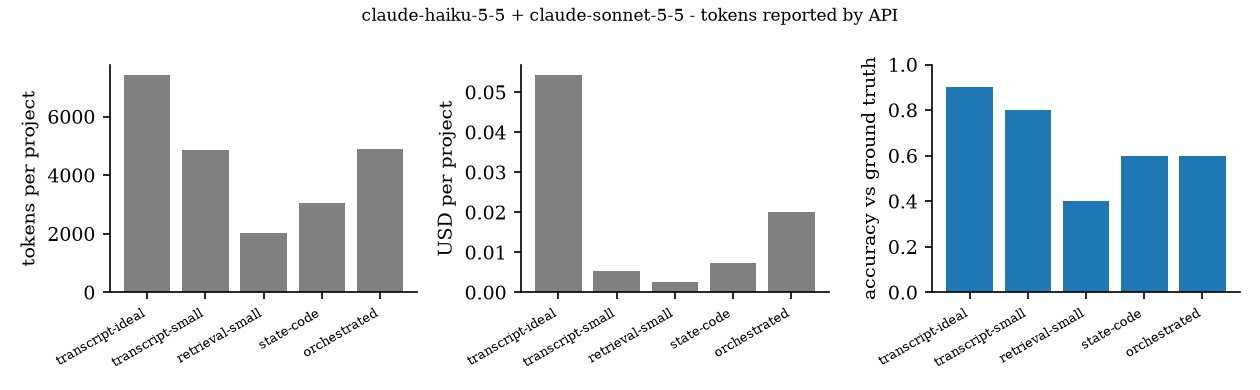
\includegraphics[width=0.98\linewidth]{figs/fig_orch_s10.png}\\[4pt]
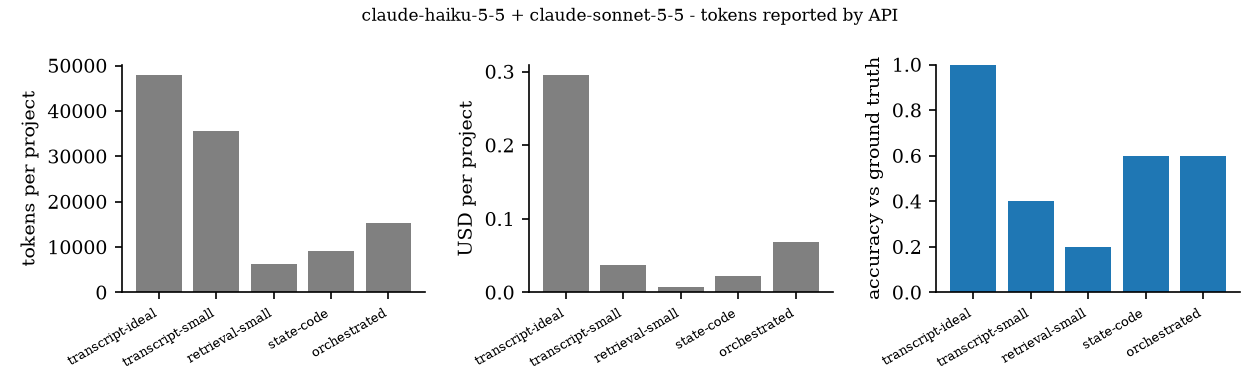
\includegraphics[width=0.98\linewidth]{figs/fig_orch_s30.png}
\caption{Orchestration benchmark: tokens per project, cost per project (assumed prices), and accuracy for each scheme at 10 sessions ($n=10$ projects, top) and 30 sessions ($n=5$, bottom).}
\label{fig:orch}
\end{figure}

\subsection{Noise stability of the decision state}
\label{sec:noise}
The orchestration results leave open why the state is less accurate and less repeatable than the transcript. We tested this offline (\texttt{qds\_sim} experiment e10, 1{,}000 simulated projects per cell, no API calls), using the correlated-noise operator of \citet{haris2026noise} as an adaptation: each evidence item (role, direction, strength) is kept with probability $\rho$ and otherwise replaced by a fresh item from the generator, so $\rho$ is the item-level correlation. (Their Eq.~7 keeps a coordinate with probability $(1+\rho)/2$, which makes $\rho=0$ a half-correlated copy; we use keep probability $\rho$ so that $\rho=0$ is independence.) The decision is $d(X)=\pm1$ and noise stability is $\mathbb{E}[d(X)d(Y)]$. The control is the additive ground-truth rule, the sign of the equal-weight sum of signed strengths.

\begin{table}[t]
\centering
\caption{Noise stability and fidelity of the decision state (simulation, 1{,}000 projects per cell). Stability is $\mathbb{E}[d(X)d(Y)]$ at item correlation $\rho=0.9$. Fidelity is the share of projects where the state's decision equals the additive rule, with exact extraction. Retest is the share of projects where two independent extractions of the same evidence (direction flipped with probability $0.18$, strength error $0.10$) give different decisions.}
\label{tab:noise}
\small
\begin{tabular}{lcccc}
\toprule
 & \multicolumn{2}{c}{10 sessions} & \multicolumn{2}{c}{30 sessions}\\
 & additive & state & additive & state\\
\midrule
Noise stability at $\rho=0.9$ & 0.73 & 0.49 & 0.72 & 0.21\\
Fidelity to additive rule, scale 1.0 & -- & 0.69 & -- & 0.48\\
Fidelity to additive rule, scale 0.1 & -- & 0.89 & -- & 0.90\\
Decision changed by shuffling the evidence, scale 1.0 & -- & 0.32 & -- & 0.50\\
Decision changed by shuffling the evidence, scale 0.1 & -- & 0.03 & -- & 0.03\\
Retest: decision differs between two extractions & 0.39 & 0.47 & 0.39 & 0.50\\
Accuracy vs clean truth under that extraction noise & 0.70 & 0.57 & 0.70 & 0.51\\
\bottomrule
\end{tabular}
\end{table}

\Cref{tab:noise} gives three results. First, the state is much less noise-stable than the additive rule, and the gap widens with history (stability $0.21$ against $0.72$ at 30 sessions), as expected of a decision that composes many non-commuting rotations. Second, and more important for \cref{sec:orch}, the state does not reproduce the additive ground truth even when extraction is exact: agreement falls from $0.89$ after one session to $0.69$ at 10 and $0.48$ at 30, which is chance, and shuffling the evidence changes the decision in half of the 30-session projects. The decision is determined mostly by the most recent items, which is the order sensitivity the framework is designed to produce, but the benchmark's ground truth is order-independent and so penalises it. Third, small rotations remove the effect: scaling strengths by $0.1$ keeps agreement near $0.90$ at every history length and the shuffle effect near $0.03$, because small rotations nearly commute. The ceiling of about $0.90$ equals the agreement of a role-weighted sum with weights $(1, 0.5, 0.5)$ with the equal-weight rule ($0.89$, 20{,}000 draws), the weights being the $y$-components of the three role axes, and not the extraction.

These results change how \cref{sec:tokens,sec:orch} should be read. The accuracy gap of the state schemes, and the failure of the stronger model to improve on the state, are largely properties of the state's form and the benchmark's order-independent ground truth, with extraction noise adding to them: even with direction flips at the observed rate the state's retest disagreement ($0.47$ to $0.50$) exceeds the additive rule's ($0.39$). The earlier code comment that the undrifted state ``matches the ground truth'' was wrong and has been corrected. A fair test of the framework needs a task whose correct answer depends on order, or a state with small rotations when order should not matter, and the choice of scale must be fixed before the data are seen. The analysis is simulation on templated evidence, uses the Bonami--Beckner operator on discrete items rather than the Gaussian operator of \citet{haris2026noise}, and says nothing about how noise-stable a Transformer is.

\begin{figure}[t]
\centering
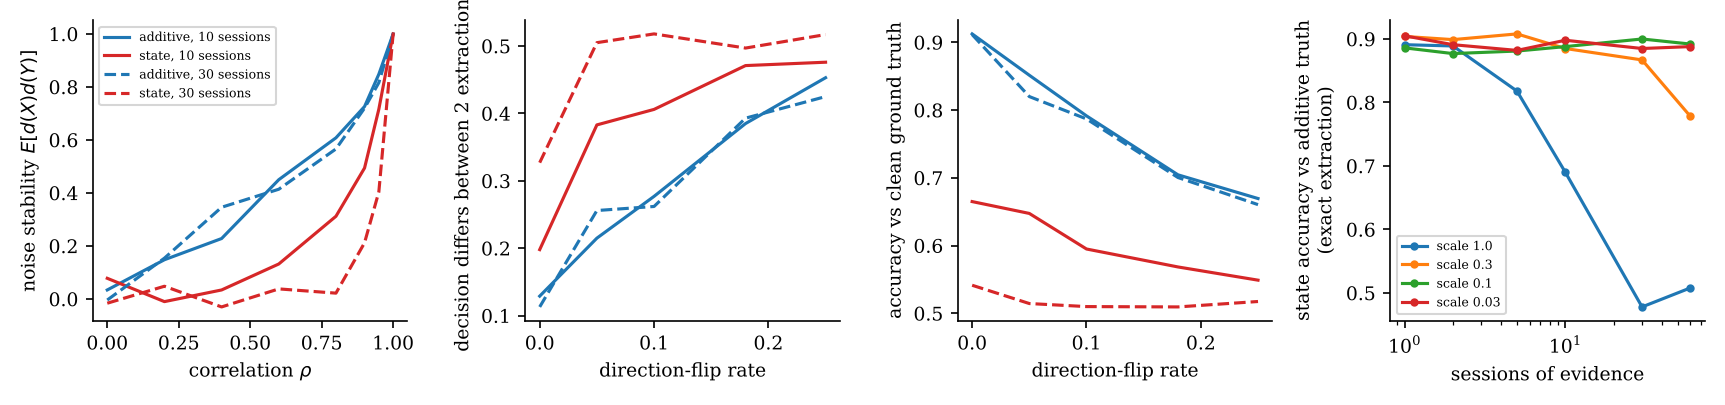
\includegraphics[width=\linewidth]{figs/fig_noise_stability.png}
\caption{Noise stability of the decision state (simulation). From left: noise stability against item correlation $\rho$; decision disagreement between two noisy extractions; accuracy against the clean additive truth under extraction noise (solid: 10 sessions, dashed: 30); and fidelity of the state to the additive rule with exact extraction against history length, for several rotation scales.}
\label{fig:noise}
\end{figure}

\section{Proposed experiments}
\label{sec:protocols}

The results above test the framework's mathematics and its fit to existing order-effect data. The timing and feedback layers make cognitive and agent-level predictions that require new data. We list them as preregistrable hypotheses.

\paragraph{H1 (decision Zeno).} Under a constant stream of weak evidence, the probability of retaining an initial judgment increases with the number of forced intermediate judgments, replicating \citet{yearsley2016} with new materials.

\paragraph{H2 (decision anti-Zeno and its null).} When evidence pressure is autocorrelated and out of step with the decision, judgments made at intervals near the pressure's correlation time accelerate abandonment relative to no intermediate judgment. When the pressure is white noise with the same total strength, the schedule has no effect beyond that of H1. Bayesian and Markov models predict no interaction between environment spectrum and schedule.

\paragraph{H3 (reminders versus commitment).} At equal cost, reminders stabilise a decision about as well as forced recommitment, but recommitment produces larger subsequent order effects.

\paragraph{H4 (delay breaks QQ).} For back-to-back questions $q\approx 0$. Inserting a delay $\Delta$ produces $|q|$ that grows on average with the drift accumulated over $\Delta$, but its size depends on where the default state lies: in simulations with random four-dimensional models, the median $|q|$ is $0.04$ when half the state has drifted and $0.08$ at near-complete drift, and in some models it is close to zero. Intervening content produces larger violations that shrink as the delay grows. The study therefore needs the content manipulation, or large samples, to have adequate power.

\paragraph{H5 (interior feedback optimum).} In multi-role tasks, outcome feedback at moderate gain delays loss of coordination; very high gain reduces coordination; lower observation efficiency lowers the optimal gain.

\paragraph{Design.} \emph{Study 1} (human, H1--H3) crosses the number of intermediate judgments (0, 1, 2, 3, 5, 11), environment type (independent versus autocorrelated pressure of matched strength), and review type (forced judgment, reminder, low-intensity rating), with roughly 1{,}000--1{,}500 online participants. Fitting must follow the two-stage procedure and state the identifiability assumption noted in \cref{sec:design}. \emph{Study 2} (human, H4) uses at least 250 participants per question order, which gives at least 90\% power for content-induced violations (\cref{sec:design}), and pairs of incompatible questions with delays of 0\,s, 30\,s, 5\,min, and 24\,h, and reports $q$, order sensitivity, and Contextuality-by-Default indices \citep{dzhafarov2016}. \emph{Study 3} (agents, H5 and memory) runs planner, critic, and executor agents on long-horizon tasks and compares, at matched memory budget, full context, summary memory, a classical Bayesian belief memory, decision-centric memory \citep{zou2026demem}, and our state memory with and without schedule and feedback control; the templated benchmark of \cref{sec:tokens} is a first, limited step toward this study.

\paragraph{Baselines and ablations.} Required baselines are a Bayesian updater with response error, a Markov random walk, the hybrid quantum--Markov open-system model \citep{busemeyer2020entropy}, the analytic hierarchy process \citep{saaty1980} as a static multi-criteria method, a long-context LLM, and the controlled Lindbladian decision maker of \citet{snow2024}. Ablations remove non-commutativity (same-axis generators), drift, environmental structure (flat $G$), reminders, and feedback.

\section{Discussion}
\label{sec:discussion}

\paragraph{What the framework offers.} It makes order, timing, and coordination explicit, gives each a closed-form quantity (conflict $C_{ab}$, drift rate $R$, coordination $I_{ab}$), and ties each to an existing, falsifiable test. The decision layer is small and inspectable: a $d$-dimensional density matrix per role and level, plus a timestamp and calibrated operators.

\paragraph{What it does not offer.} A density matrix stores a leaning and its uncertainty, not the content of a decision or the reasons for it. The framework therefore complements retrieval and decision-centric memory rather than replacing the context window. Its memory cost is $d^2-1$ real numbers per decision, and \cref{lem:recip} shows that $d$ must exceed two for realistic questions; multi-attribute decisions represented by tensor products grow exponentially, so dimensionality must be chosen from data, for example by singular value decomposition of joint response tables, the same tool used to identify independent mode pairs in temporally multiplexed optical systems \citep{li2020temporal}.

\paragraph{Limitations.} Our empirical evidence is a reanalysis of existing data, simulations of the model, and one templated token benchmark with a real language model; we have not yet run the human studies in \cref{sec:protocols}, and the agent-level evidence does not show that the state memory matches full-context decision quality. The overlap law is a weak-coupling result, so claims are restricted to regimes where stored decisions remain likely to survive. The cognitive interpretation of $G(\omega)$ and $\omega_a$ requires operational validation. The linear-Gaussian surrogate is approximate for single decisions. The order-free classical model fitted one laboratory data set best, so quantum structure is not always needed. Classical mechanisms can also satisfy the QQ equality (\cref{prop:carry}; \citealp{kang2026}), and our model-recovery simulations show that order-effect data discriminate weakly, so support for the framework must come from the joint pattern of H1--H5, not from the equality alone. The design analyses in \cref{sec:design} use synthetic data generated from the models themselves; they establish that the analyses work and how large the studies must be, not that the hypotheses hold. The token and orchestration benchmarks use templated evidence, an additive ground truth, one model pair, small numbers of projects (5 to 30), and assumed prices; the rescaled-state result is tuned post hoc; and in the orchestration pilot the state schemes were less accurate than the large-model transcript, answering from the state with a stronger model added no accuracy, and extraction noise changed decisions between runs. The noise-stability analysis (\cref{sec:noise}) shows that the state with unit rotation scale does not reproduce an order-independent additive rule even with exact extraction, so the accuracy comparison against an additive ground truth is not a fair test of the framework; a task with order-dependent truth has not been run. Finally, several system papers we draw on are recent preprints whose claims have not yet been peer reviewed.

\begin{table}[t]
\centering
\caption{Status of the main claims.}
\label{tab:claims}
\small
\begin{tabular}{p{0.45\linewidth}p{0.47\linewidth}}
\toprule
Claim & Status\\
\midrule
Commuting criteria give no order effects; conflict $=2\sin\varphi$; rank-one answers force reciprocity; flat environment gives schedule-independent drift & Mathematical facts (\cref{prop:commute,prop:comm,lem:recip,prop:null}); symmetric carry-over satisfies QQ (\cref{prop:carry})\\
Planned analyses recover generating parameters; 250 per order gives $\ge 90\%$ power for content-induced violations & Simulation results on synthetic data (\cref{sec:design})\\
State memory uses fewer tokens than a transcript memory at 10 and 30 sessions & Supported in a templated benchmark (\cref{tab:tokens}); retrieval is cheaper, and decision-quality parity is not shown\\
State pipeline is cheaper than a large model re-reading the transcript & Supported at pilot scale with assumed prices (\cref{tab:orch}); not cheaper than a small model doing so at 10 sessions or with rare answers\\
State decision reproduces an order-independent additive rule & Not supported at unit rotation scale (agreement $0.69$ at 10 sessions, $0.48$ at 30, exact extraction; simulation, \cref{tab:noise}); about $0.90$ at scale $0.1$\\
State pipeline matches transcript accuracy; a stronger model answering from the state improves it & Not supported at pilot scale (\cref{tab:orch}): lower point estimates, identical decisions with and without the stronger answerer\\
Overlap law, Zeno and anti-Zeno effects; feedback prevents entanglement sudden death & Physics results \citep{kofman2005,fischer2001,yamamoto2008pra}, used here by analogy\\
QQ equality holds in survey data; rank-one models fail & Supported by reanalysis (\cref{tab:qq}) and \citet{wang2014}\\
Intermediate judgments slow opinion change & Supported in one paradigm \citep{yearsley2016}\\
Decision anti-Zeno; reminder--commitment equivalence; delay-induced QQ violation; interior feedback optimum in people or agents & Hypotheses requiring data (H2--H5)\\
Non-classical (entanglement-like) correlations between roles & Not claimed; future work only\\
\bottomrule
\end{tabular}
\end{table}

\section{Conclusion}
We proposed a quantum-probability decision state for role-aware agents and filled three gaps in it with results from quantum cognition, dynamical decay control, and quantum feedback networks. The resulting framework explains when order matters (non-commuting criteria with answer subspaces of rank at least two), predicts when timing matters (only in structured information environments, with both Zeno and anti-Zeno regimes), and shows how feedback can keep coupled roles coordinated. A reanalysis of published survey data supports the order layer and rules out the simplest one-dimensional representations. The timing and feedback layers make specific, falsifiable predictions, and we have set out the experiments needed to test them. In a first benchmark with a real language model the state memory reduced tokens relative to a transcript, increasingly so for longer histories, but did not yet match its decision quality, so the practical case for the memory remains open. A pilot orchestration run with a stronger answering model did not close it: the state pipeline was cheaper than a large model reading the transcript, but not than a small model at short histories or with rare answers, and answering from the state added cost without accuracy. A noise-stability analysis attributes much of the accuracy gap to the state's non-commuting form rather than to the language model, so a fair test needs order-dependent ground truth.

\section*{Code availability}
The \texttt{qds\_sim} package contains the library, the test suite, and one script per analysis in this paper (reanalysis of published data, H1--H5 design simulations, model recovery, the mock agent harness, the token and orchestration benchmarks, the hierarchy pilot, the noise-stability analysis, and an accuracy-evaluation script); result files for every run reported here are included. The repository is available at \texttt{https://github.com/lalit-aditya/quorum-state}.

\section*{Acknowledgements}
The author thanks the researchers who made the data and methods used here publicly available, in particular the authors of the published order-effect data sets reanalysed in \cref{sec:results} and the authors of the noise-stability framework adapted in \cref{sec:noise}. The simulations and figures were produced with the open-source NumPy, SciPy and Matplotlib libraries, and the token and orchestration benchmarks were run through the Anthropic API.

\bibliographystyle{unsrtnat}
\bibliography{refs}

\end{document}
